\documentclass{sig-alternate}
\usepackage[utf8]{inputenc}
\usepackage{times}
\usepackage{gensymb}
\usepackage{epsfig}

\begin{document}
\conferenceinfo{CIDR '17}{January 8-11, 2017, Santa Cruz, CA, USA}
\newcommand{\smallitem}[1]{\vspace{1em}\noindent\textbf{#1}}
\newcommand{\smallitembot}{\vspace{1em}\noindent}



\title{Grounding Big Data with Data Context Services}
\numberofauthors{3}
\author{
Groundlings
}

\maketitle

\section{From Metadata to Context}
The open-source Big Data movement, spearheaded by Apache Hadoop, is often discussed in terms of changes in usage: the ``three V's'' of data being captured, and the agile working style typified by ``schema-on-use'' and polyglot programming models.

Much less widely discussed is a profound shift toward a decoupled software architecture. Traditionally, database systems were consumed as monolithic stacks of component functionality, regardless of how well-factored they were under the covers. A DBMS included a consistent storage engine, a metadata catalog, a dataflow engine, a language compiler and optimizer, an execution scheduler/runtime, and facilities for data ingest and queueing.  Nearly all of these components are independent and swappable in today's Big Data stack. Moreover, there are multiple choices for most of these components in wide use today. The decoupled architecture is healthy for innovation and specialization, and has been embraced by both developers and customers.

One negative side-effect of this diversity is the lack of an agreed-upon service to register metadata for these components. The only widely-used solution is the Hive Metastore, which serves simple relational schemas---a dead end for Variety. As a result, most ``Data Lake'' projects lack even the most basic information; typically it is not even possible to discover what is being stored. 
For emerging Big Data customers and vendors, this Big Metadata problem is hitting a crisis point.  Two serious problems emerge.

The first is poor productivity.
%The promise of the Data Lake is that a diversity of data can be easily captured, and then harnessed by analysts for value. 
In the absence of metadata, analysts are often unable to discover what data exists, much less how it may have been previously parsed, structured, cleansed and analyzed by peers. ``Tribal knowledge'' in an organization is the standard method for disseminating this information today. Clearly this does not scale, leading to wasted work and lost opportunities for analysts to build on the data and analysis known to others.

The second problem is governance risk. Data management necessarily entails recording governance information: who accesses data, what they do with it, where they put it, and how it gets consumed downstream. 
%In some cases this governance metadata is used to enforce policy (e.g.\ access control for Personally Identifiable Information); in others it is logged to support audits for compliance (e.g.\ in the Basel Committee on Banking Supervision). 
In the absence of a standard place to store and access this information, it is impossible to enforce policies and/or audit behavior. As a result, many administrators marginalize their Big Data stack as a playpen for non-sensitive data.

In our diverse experiences in industry, the authors have seen a pressing need for a common service layer to let Big Data components ``write down'' and share metadata information in a flexible way. The effort in this paper began by addressing that need.

\subsection{Metadata Crisis? Context Opportunity.}
The lack of a Big Data metadata service is not just a crisis; it is also a clean-slate opportunity to rethink design and usage. Storage economics and the simplicity of schema-on-use suggest that the Data Lake movement could go much farther than Data Warehouses in enabling diverse, widely-used central repositories of data.  If we view metadata more broadly, could a unified solution address a much broader set of goals than Data Warehouses? We can explore that notion along three axes:

\smallitem{Data.} A schema-on-use world is inherently relativistic. Data does not have \emph{inherent} structure and meaning; rather, the structure is imposed post hoc---sometimes for general usage, sometimes for a specific task.  This means that the ``description'' of a collection of data depends not only on its original form, but on the (many) ways it is transformed for use over time.  

\smallitem{Code}. Data is transformed by code, which becomes a necessary aspect of data description. Transformation is only one kind of data-centric code. There is also code that produces new data: analysis routines, statistical models, and outbound services like recommenders and ad systems. Data \emph{lineage} is a natural byproduct of code, relating it to data sources and outputs. Code also brings along data of its own: training data, model parameters, configuration files, etc. This is not the data of record in an organization; it is an aspect of the code itself. Code management brings its own requirements, notably information on versions, authors and testing.  
%With code and data versioned over time we can envision robust reproducibility of experiments---a feature of interest in areas including hypothesis testing (e.g. A/B tests) and in scientific verification.  

\smallitem{Usage}. In modern agile analytic environments, iterations of exploration, experimentation and (re)deployment of automated pipelines are daily activity. Ironically, today's Big Data software is not well-designed for enabling analysis of its own use. If people learn by doing, then the tribal knowledge of an analytic organization should be visible in its usage logs. Intelligent analytic software could take great advantage of these logs to augment and accelerate human activity and intelligence. Like all software usage logs, analytics logs are themselves big, diverse data.

\smallitembot
The enhanced functionality needed for this layer of the modern Big Data stack goes well beyond traditional metadata management. We refer to it as \emph{Data Context} services. Context refers to the full gamut of peripheral information that informs your analysis: what data and code do you have, where is it stored, when does it get used, who knows about it, and how does it change over time?  

\section{Ground: Scenarios and Design}
We are building an open-source data context service we call \emph{Ground}---a foundation for the broad data context agenda sketched above. 
The goal of Ground is to serve as a central model, API and repository for capturing the broad context in which data gets used. In designing Ground, our intent is to address practical problems for the Big Data community in the short term, and open up opportunities for research and innovation as well.

\subsection{Scenarios}
To illustrate the benefits of data context, consider the following scenario. It is only modestly futuristic: there are applications that do some of these things today, but could do far more if they had broader context.

\textbf{Idea 1: Intelligent Business Intelligence.}  Janet, an analyst at a major bank, believes that customers' social network behavior can help explain their likelihood of closing their account (churning). Evaluating this hypothesis requires a pipeline of stages: data acquisition, transformation and analysis. 
% Intelligent applications are emerging for each of these tasks today, which make suggestions to users. All could benefit from a more comprehensive service for data context, as we illustrate below.

Janet 
% plans to purchase a social media ``firehose'' feed for her analysis. To start, though, she 
begins by downloading a small sample of a social media feed from a free API into the data lake. Her data catalog application notifies her that the bank has a large dataset of very similar data from the previous month. She finds this sufficient for her purposes; no need to pay for another feed. She then begins searching the catalog for historical data on customer churn: what is available, and who has access to it?  As she explores candidate schemas and data samples, she is notified that one of her colleagues has access to many of these datasets, and has previously joined one of them with weather data. She decides to start with that dataset as well, and compare notes with her colleague later on.  In this scenario, the catalog application was particularly successful because it had access to broad context: not just a large corpus of data, but structured schemas for that data based on prior (schema-on-)use, as well as usage data capturing relationships between users, data and actions.

Once Janet chooses particular datasets to focus on, she begins to prepare them for analysis using a data wrangling application. As is typical, the social media feed is semi-structured and deeply nested; the application suggests unnesting attributes and pivoting them into tabular form.  The application then makes her aware of a number of posts from a GPS location at a great distance from any of  the bank's branches. Janet is given suggestions to generate new columns derived from the social text using code for entity extraction and sentiment analysis written by her data science colleagues. She is warned that certain attributes of the customer churn data were marked confidential by another analyst, and should perhaps be masked. Finally, when she is ready to join the social media names against the bank customer names, the application helps identify and standardize the join keys appropriately. The data wrangling application benefited from context it would not have seen as an isolated component: reference data like geographic distributions of branches, repositories of data science routines, and the analytic context that the datasets being wrangled came from the data lake with security annotations. \emph{Would be nicer to get an analytic context about Janet's behavior.}

Armed with a tidy table of hundreds of columns joined together, Janet opens her chosen BI charting application. She plans to cube the data set along various features of users and social media behavior, assessing churn rates in different categories. Given the richness of her wrangled table, the resulting number of potential charts is enormous. Fortunately her BI tool has automated features to recommend charts of interest, and focuses on breaking down the data hierarchically along time, space, and the extracted sentiment scores and bank-specific entity features; it omits customer names and the attributes marked confidential.  Here again the BI tool benefits from broad context: it sees the lineage from the data wrangling application and knows what features were results of complex computations; it also sees the confidentiality markings from the catalog application two steps upstream.
% ; these tools use intrinsic properties of their input data today~\cite{jeffheer}. To work better, they could benefit from the lineage of transformations that created their input---in our case recognizing the presence of social media data at the source, and recommending charts that were chosen for visualizing other outputs of social media datasets.
%If interesting patterns emerge in the data visualizations, the analyst may recommend decisions to the organization: e.g. to deploy customer service representatives to respond on social media, or to have the data science team incorporate social media feeds into more sophisticated predictive models for churn.


% \emph{A number of new applications for data analysts have begun to capture data context and provide assistive intelligence as described above, but they currently have no way to share that information.  Hence the scope of their context is limited to what they see at their inputs. Broadly-adopted data context services are key to expanding the intelligence of these applications, harnessing data and computation to improve analyst productivity.}


\emph{\textbf{Idea 2: Model training and serving.  Joey to fill in?} 
% The previous example focused on relatively simple exploratory data analysis. 
Data context can bring similar benefits to the kinds of predictive services that hardcore data scientists build and deploy live in modern hosted applications.  Large-scale predictive services like recommender systems and driving instructions rely on data scientists and engineers working in agile development cycles.  The services are based on serving results from models; the models themselves are periodically trained off of features extracted from data. Data and features evolve over time. Meanwhile, there should be a virtuous cycle of model training, serving and experimentation.  Want to improve this cycle. Want to be able to run new models on old traces (cite Johann's paper). Want to incorporate new models in debug mode in production. Want to be able to reward staff for improving models. Want to reallocate staff when the benefit of experimenting with the model no longer justifies the effort.}

\emph{\textbf{Idea 3: A Pragmatic example in existing Hadoop workflows.  LinkedIn or Navigator customer story?}  Maybe take Idea 1 and make it less about assistive features, more about lost lineage across HDFS, Trifacta, Hive and Tableau?}

\subsection{Design Requirements}
Three key design requirements for Ground arise naturally blah blah... KEY: MAKE A SIMPLE DECISIONS TODAY 
THAT GUARANTEES YOU CAN MAKE A WIDE RANGE OF DECISIONS AND INNOVATIONS TOMORROW.

\emph{Joey: we should have a set of requirements here. List them, Justify them, Argue that they are not well-solved by other solutions.  Also make them interesting.}

\smallitem{Model-Agnostic.} In most Big Data stacks, data arrives in many formats and data models, and is transformed into many others using a variety of tools and languages. For a data context service to be broadly adopted, it cannot impose its own opinions on how data is modeled. As a corollary, it cannot be prescriptive about how metadata is modeled. A key challenge in Ground is to design a core metamodel that easily captures both generic information that applies to all data context, and specific forms of information that exist in different data models, applications, and usage.  \emph{Reduce friction. Enable agile evolution over time.}

\smallitem{Immutable.} Context goes across time, bro.  This is interesting!

\smallitem{Scalable.}  This is a function of the storage beneath, to a large extent. But still, the API dispatch, consistency model, and other aspects of the specification should not preclude the management of enormous volumes of metadata.

\smallitem{Politically Neutral.}  While not a technical design requirement per se, we note that metadata services have to be Switzerland to be successful.  The goal is for customers to adopt them without fear of lock-in, and applications to work with them without fear of being ghettoized. Vendor-centric solutions in this space have traditionally raised concerns on those fronts; this is perhaps why the MDM vendors have not been successful in the market. Open source is not a panacea; customers have to believe that the code committers and project leaders do not have financial or political incentives to behave against their interests.  

\vspace{1em}
These are all opportunities to go beyond solving the current crisis, providing for a better future.  

\section{Architecture of Ground}
\begin{figure}
\center
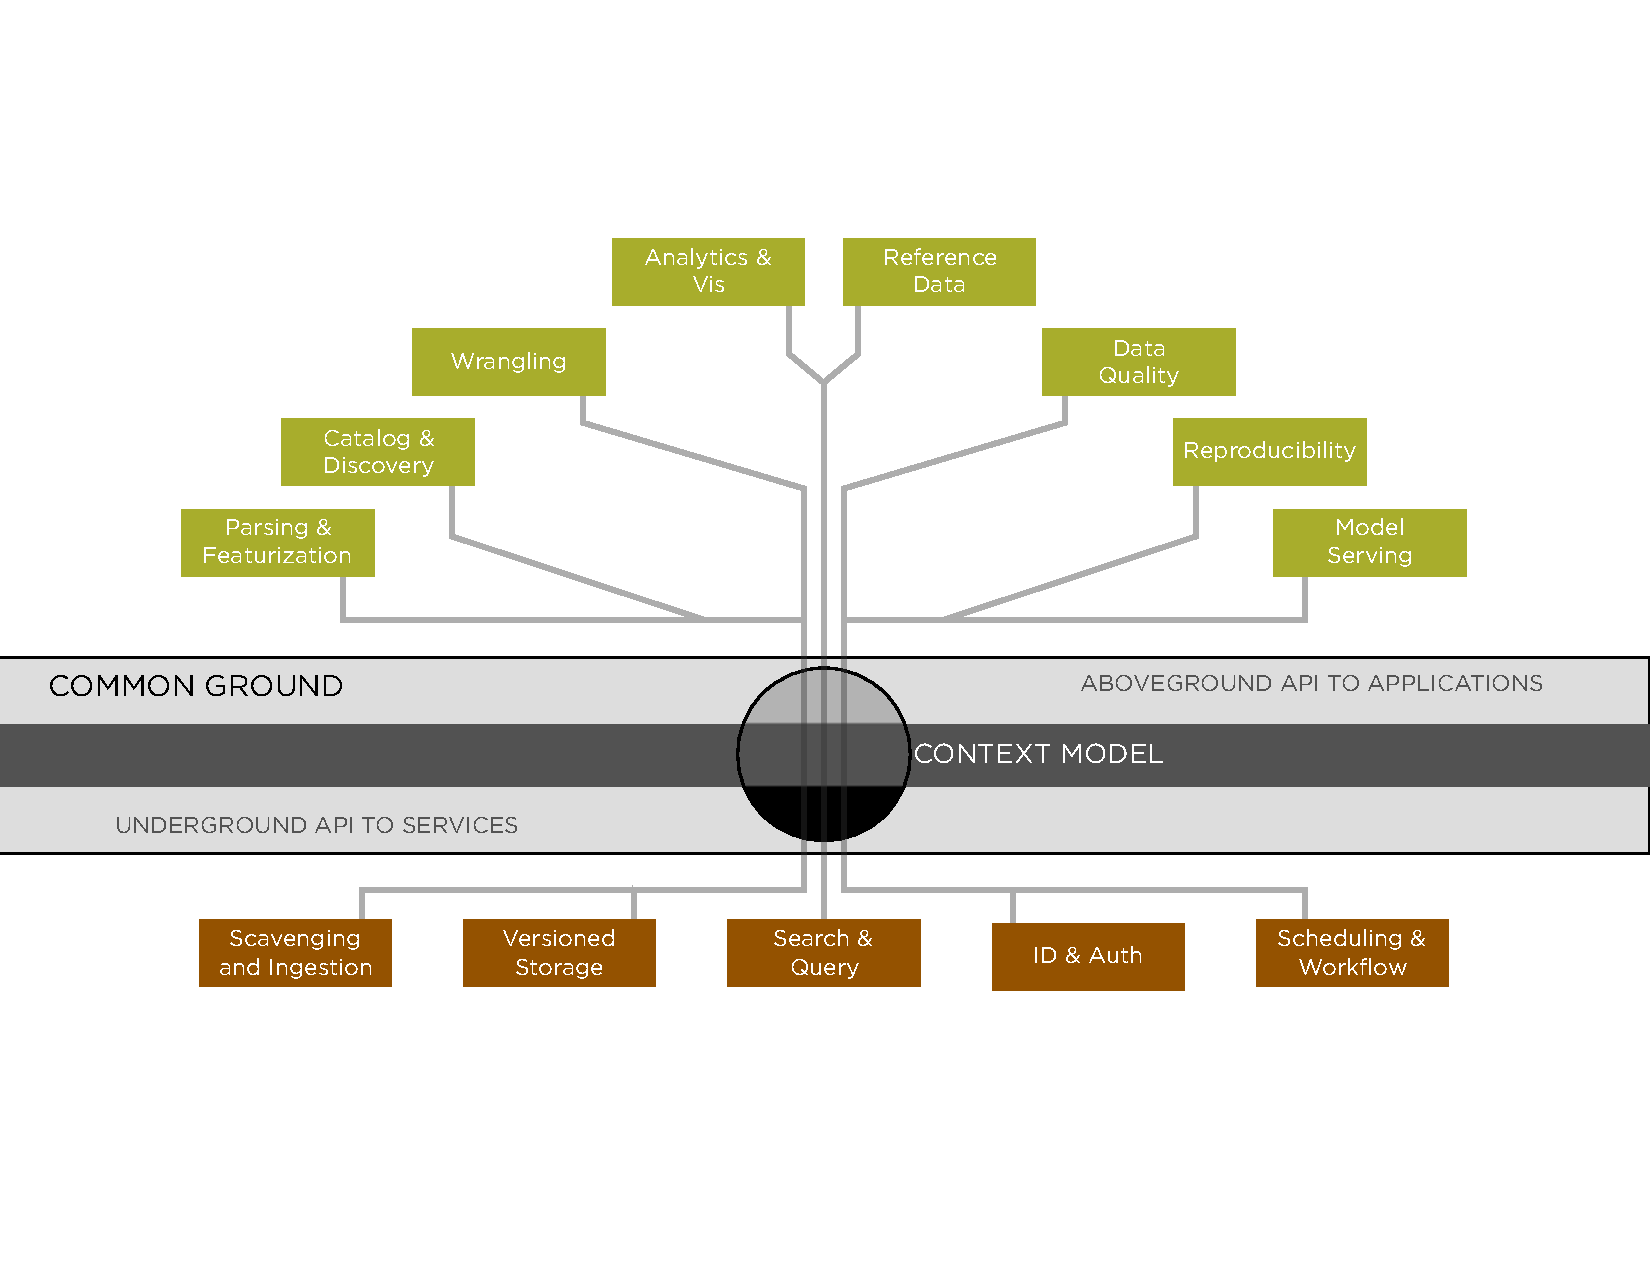
\includegraphics[width=0.7\linewidth]{groundarch.pdf}
\end{figure}

\subsection{Common Ground: A Metamodel}
\subsection{Underground Services}

\section{Prototype Evaluation}
Functionality and Performance/Scale.

Functionality: well, we've started building out a few things and they went well.  Apiary and Grit.

What about performance? Here we ran into some bottlenecks with the widely-used storage systems in the field.  This merits more attention.

\section{Challenges for the community}
\end{document}
